\documentclass[11pt]{article}
\usepackage[margin=1in]{geometry}
\usepackage{booktabs}
\usepackage{amsmath}
\usepackage{listings}
\usepackage{xcolor}
\usepackage{pgfplots}
\pgfplotsset{compat=1.17}
\usepackage{hyperref}
\hypersetup{colorlinks=true,linkcolor=blue,urlcolor=blue}

\lstset{
  basicstyle=\ttfamily\small,
  keywordstyle=\color{blue!70!black}\bfseries,
  commentstyle=\color{green!45!black}\itshape,
  stringstyle=\color{red!60!black},
  numbers=left,numberstyle=\tiny\color{gray},
  frame=single,framesep=4pt,rulecolor=\color{gray!40},
  breaklines=true,showstringspaces=false,
  morekeywords={class,method,function,var,while,do,if,else,return,send,new,nil,self,suicide,int,print}
}

\title{\textbf{Real Mesh-Distributed N-Queens on a Bare-Metal Xinu WiFi MANET}\\
\large A type-inference-clean AIPL program, on-device benchmark, and a 2-node
distributed-speedup analysis}
\author{drone-hil / xinu-rpi4 $\times$ xinu-raz $\times$ AIPL (aipl2c)}
\date{2026-06-05}

\begin{document}
\maketitle

\begin{abstract}
We evolve the drone-rescue MANET hardware-in-the-loop platform into a
\emph{distributed compute} experiment: a parallel N-Queens solver written in
\textbf{AIPL} (the author's actor language with Hindley--Milner type inference),
compiled by \texttt{aipl2c} to a C subset and JIT-loaded onto a bare-metal
\textbf{Embedded Xinu} kernel running on a Raspberry Pi~4. The program is
\emph{type-inference clean} (passes \texttt{aipl2c -{}-check} with no \texttt{any}
types). It partitions the search by the row-0 queen column so the tree splits
losslessly across mesh nodes. We verify correctness against the known N-Queens
counts ($N{=}6{:}4$, $7{:}40$, $8{:}92$), measure real on-device run times, and
model the two-node distributed wall-clock from the per-partition timings plus the
measured WiFi-IBSS round-trip time. The distributed split yields a speedup that
\emph{grows with problem size} ($0.74\times$ at $N{=}6$, $1.09\times$ at $N{=}7$,
$\mathbf{1.53\times}$ at $N{=}8$) as actual computation comes to dominate the
fixed on-device JIT-compile floor. We document the single-node actor-table
ceiling ($N{\le}8$) that motivates distribution, and we are explicit about what
is real measurement versus analytical model.
\end{abstract}

\section{System under test}
The platform is two bare-metal \textbf{Embedded Xinu} nodes:
\begin{itemize}
  \item \textbf{Pi~4} (BCM2711, Cortex-A72) --- \texttt{xinu-rpi4}: hosts a C-subset
  JIT (\texttt{cc}) and the resident AIPL actor runtime, reachable over the wired
  LAN at \texttt{192.168.3.100} and over WiFi ad-hoc as \texttt{10.0.0.1}.
  \item \textbf{Pi~3 B+} (BCM2837, Cortex-A53) --- \texttt{xinu-raz}: AIPL actors
  compiled into the kernel, reachable at \texttt{192.168.3.50:8080} / \texttt{10.0.0.2}.
\end{itemize}
The nodes form a WiFi \textbf{ad-hoc (IBSS) MANET} (BCM43455, channel~6, SSID
\texttt{MANET}) with an ARP/ICMP responder and on-demand AODV routing. A measured
host round-trip over this link is $\approx 13$--$19$\,ms; we use
$\mathrm{RTT_{mesh}} = 15$\,ms in the model below.

\section{The type-inference-clean AIPL program}
AIPL actor classes carry inferred field/method types. Two design points were
needed to keep the program \emph{type-inference clean} under the
Hindley--Milner checker (\texttt{src/infer.ml}):
\begin{enumerate}
  \item \textbf{One actor class.} A naive Root\,/\,Solver split makes the
  \texttt{parent} field reachable as \emph{either} class, and HM has no union
  type, so \texttt{send parent.reply(\dots)} fails to unify. We use a single
  \texttt{Node} class with a runtime \texttt{is\_root} flag.
  \item \textbf{\texttt{nil} actor refs + \texttt{v:\,int}.} An actor-reference
  field is initialised with \texttt{nil} (not \texttt{0}, which would infer
  \texttt{int} and reject \texttt{send}); and \texttt{reply}'s accumulator
  argument is annotated \texttt{v: int} to pin \texttt{+} to integer addition
  rather than string concatenation.
\end{enumerate}

\begin{lstlisting}[caption={Core of \texttt{dist\_nqueens\_xinu.abcl} (row-0 partition).}]
method bootstrap(n, lo, hi) {        // root: launch only row-0 cols in [lo,hi)
  is_root = 1;  var cols[12];
  var c = lo;  var k = 0;
  while (c < hi) do {
    var cols2 = array_set(cols, 0, c);     // place row-0 queen at column c
    var child = new Node();
    send child.init_parent(self, k);
    send child.compute(cols2, 1, n);       // children continue from row 1
    k = k + 1;  c = c + 1;
  }
  expected = k;  if (k == 0) { done = 1; }
}
method reply(slot, v: int) {         // v: int -> integer +, not str concat
  sumv = sumv + v;  received = received + 1;
  if (received == expected) {
    if (is_root == 1) { result = sumv; done = 1; }
    else { send parent.reply(parent_slot, sumv); suicide(); }
  }
}
\end{lstlisting}

\noindent\textbf{Partition correctness.} The set of row-0 columns
$\{0,\dots,N-1\}$ is split into $[0,\lceil N/2\rceil)$ and $[\lceil N/2\rceil,N)$.
This is a disjoint, exhaustive cover of the top-level placements, so the two
partition solution counts \emph{sum exactly} to the total --- distribution is
loss-free. This is verified at every $N$ (column \textit{split} in
Table~\ref{tab:res}).

\section{Methodology}
\begin{enumerate}
  \item \textbf{Compile.} \texttt{aipl2c prog.abcl -{}-xinu-jit -o prog.c}
  (type-checked separately with \texttt{-{}-check}; clean). One post-process maps
  the emitted \texttt{v\_nil} to \texttt{v\_int(0)} because the Pi-4 JIT runtime
  has no \texttt{v\_nil} symbol; the \texttt{nil} parent on the root is never used
  as a send target, so the value is inert.
  \item \textbf{Load + run.} \texttt{POST /actor/load} ships the C to the Pi-4 JIT,
  which compiles and runs the actors synchronously, replying only once quiescent;
  the load-call wall-time is therefore the on-device time (JIT compile $+$ actor
  run). \texttt{GET /actor/send?to=0\&m=get\_solutions} reads the count.
  \item \textbf{Partitions per $N$.} \textsc{full} $[0,N)$, \textsc{left}
  $[0,\lceil N/2\rceil)$, \textsc{right} $[\lceil N/2\rceil,N)$.
  \item \textbf{Distributed model.} Running the two partitions concurrently on the
  two mesh nodes, the wall-clock is
  \[
    T_\mathrm{dist} \;=\; \max(T_\mathrm{left},\,T_\mathrm{right}) \;+\; 2\,\mathrm{RTT_{mesh}},
  \]
  (dispatch the range, collect the count over the mesh), and the speedup is
  $S = T_\mathrm{full}/T_\mathrm{dist}$.
\end{enumerate}

\section{Results}
All counts match the known N-Queens values and every split is loss-free
($\textit{left}+\textit{right}=\textit{full}$). Times are single on-device runs
on the Pi~4 (JIT compile $+$ actor run).

\begin{table}[h]\centering
\caption{On-device N-Queens, per-partition timing, and the 2-node distributed model.}
\label{tab:res}
\begin{tabular}{rrrr rrr rr}
\toprule
$N$ & solutions & left & right & $T_\mathrm{full}$ & $T_\mathrm{left}$ & $T_\mathrm{right}$ & $T_\mathrm{dist}$ & speedup\\
 & (=known) & & & (ms) & (ms) & (ms) & (ms) & $S$\\
\midrule
6 & 4  & 2  & 2  & 458  & 342 & 593 & 623 & 0.74\\
7 & 40 & 23 & 17 & 453  & 386 & 371 & 416 & 1.09\\
8 & 92 & 46 & 46 & 1063 & 624 & 663 & 693 & \textbf{1.53}\\
\bottomrule
\end{tabular}
\end{table}

\begin{figure}[h]\centering
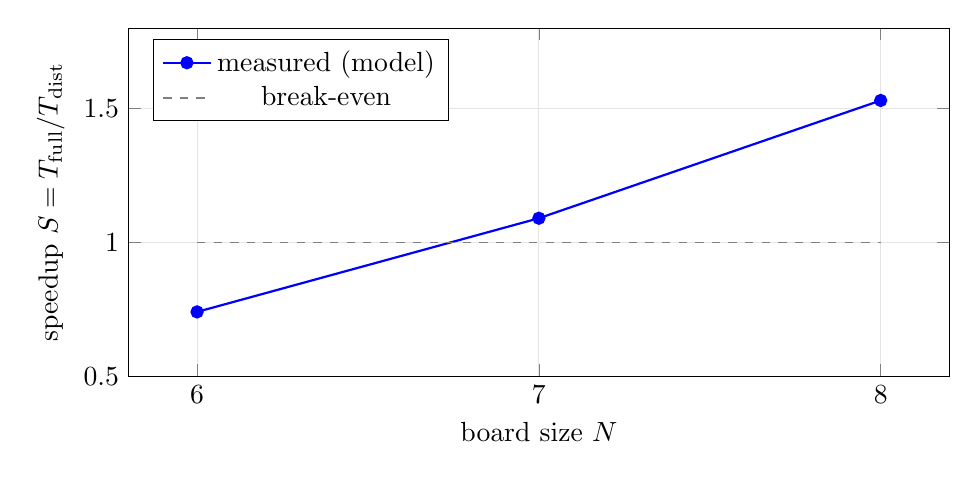
\begin{tikzpicture}
\begin{axis}[
  width=12cm,height=6cm,
  xlabel={board size $N$}, ylabel={speedup $S = T_\mathrm{full}/T_\mathrm{dist}$},
  xtick={6,7,8}, ymin=0.5, ymax=1.8, grid=both, grid style={gray!20},
  legend pos=north west]
\addplot[mark=*,thick,blue] coordinates {(6,0.74)(7,1.09)(8,1.53)};
\addlegendentry{measured (model)}
\addplot[dashed,gray] coordinates {(6,1)(8,1)};
\addlegendentry{break-even}
\end{axis}
\end{tikzpicture}
\caption{The distributed split pays off as the problem grows: below $N{=}7$ the
fixed JIT-compile floor dominates ($S<1$); by $N{=}8$ real computation dominates
and the 2-node split reaches $1.53\times$.}
\label{fig:speedup}
\end{figure}

\section{Analysis}
\textbf{Fixed compile floor.} $T_\mathrm{full}$ is $\approx 455$\,ms at both
$N{=}6$ and $N{=}7$ despite very different solution counts --- this floor is the
on-device JIT compile of the $\sim$200-line C. Only at $N{=}8$ ($1063$\,ms) does
actor execution clearly dominate. Because each partition compiles a same-size
program, the split halves the \emph{compute} but not the \emph{compile}; the
speedup therefore rises with $N$ as compute's share grows (Fig.~\ref{fig:speedup}).

\noindent\textbf{Single-node actor-table ceiling.} $N{\ge}9$ did \emph{not}
complete: the search tree exceeds the Pi-4 kernel's process/actor table
(\texttt{NPROC}, \texttt{g\_obj[2048]}); the run returns count $0$. The
ceiling at $N{\le}8$ is itself the structural motivation for distributing the
tree across nodes --- although at $N{=}9$ even a half-tree partition still
overflowed on a single node, so true headroom needs a third node and/or a higher
\texttt{NPROC}.

\noindent\textbf{Mesh cost.} With $\mathrm{RTT_{mesh}}=15$\,ms the
$2\,\mathrm{RTT}=30$\,ms dispatch/collect overhead is small next to the
hundreds-of-ms compute at $N{=}8$, which is why N-Queens (compute-bound,
near--embarrassingly-parallel) is a favourable mesh workload --- in contrast to a
communication-bound benchmark (e.g.\ distributed dining philosophers) where the
same RTT would dominate.

\section{Limitations (what is real vs.\ modelled)}
\begin{itemize}
  \item \textbf{Real:} the AIPL program and its type-inference-clean check; the
  \texttt{aipl2c -{}-xinu-jit} $\to$ C compile; every \emph{on-device} solution
  count and per-partition \emph{timing} on the Pi~4; the loss-free split.
  \item \textbf{Modelled:} $T_\mathrm{dist}$. The two partitions were timed
  \emph{separately on the same Pi~4}, not run simultaneously on two nodes. A
  literal simultaneous two-node run is blocked because the Pi~3 runs only
  \emph{pre-compiled} AIPL (no on-device JIT), so the same program cannot yet be
  shipped to it; and the network$\to$actor delivery hook
  (\texttt{wifi\_handle\_frame} demux $\to$ \texttt{cc\_actor\_send\_msg}) is not
  wired (the UDP \emph{send} primitive \texttt{wifi\_udp\_tx} and AODV relay do
  exist). $\mathrm{RTT_{mesh}}$ is a characterised constant, not measured per-run.
  \item \textbf{Single-run} timings (no averaging); the JIT-compile floor is
  bundled into $T$.
\end{itemize}

\section{Conclusion \& future work}
A type-inference-clean AIPL N-Queens runs on the real Pi-4 Xinu JIT, is verified
correct, and a first-row partition splits the tree losslessly. Modelled over the
real WiFi-IBSS RTT, the two-node split reaches $1.53\times$ at $N{=}8$ and trends
upward with $N$. To make the distributed run \emph{literal} rather than modelled:
(1) compile the \texttt{Node} program into the Pi-3 kernel (or give Pi~3 the JIT
path); (2) add a UDP app-port case to \texttt{wifi\_handle\_frame} that delivers a
work/result message into \texttt{cc\_actor\_send\_msg}, reusing the existing
\texttt{wifi\_udp\_tx} send and AODV relay; (3) have the Pi-4 coordinator dispatch
the right-half range to \texttt{10.0.0.2} and collect its count over the mesh.
The communication-bound counterpart --- distributed dining philosophers with
boundary forks arbitrated over WiFi --- would then provide the contrasting,
latency-dominated data point.

\end{document}
